\documentclass[]{beamer}

\usepackage{graphicx}% Include figure files
\usepackage{dcolumn}% Align table columns on decimal point
\usepackage{float}
\usepackage[separate-uncertainty=true,multi-part-units=single]{siunitx}
\usepackage[english]{babel}
\usepackage[]{natbib}



\title{Asteroseismology of KIC 7107778: a binary comprising almost identical subgiants}
\author{Miles Lucas}
\institute{Department of Physics and Astronomy \\ Iowa State University}

%\usetheme{lucid}
\begin{document}
	\frame {
		\titlepage
	}
	\frame {
		\frametitle{Introduction}
		Binary systems provide a good laboratory for studying stellar evolution due to their convenient constraints on metal abundance and age. Asteroseismology allows new ways to study binaries that previously could not due to being unresolved or non-eclipsing. The study of KIC 7107778 by Li and Bedding will show the power of asteroseismology in a very unique binary system. 
	}
	\frame {
		\frametitle{Conclusions}
		\begin{enumerate}
			\item<1-> KIC 7107778 is comprised of two subgiant stars with overlapping, solar-like power spectra
			\item<2-> The estimated stellar parameters of these stars show that they are nearly identical
		\end{enumerate}
	}
	\frame{
		\frametitle{KIC 7107778}
		Interesting features of this binary system
		\begin{itemize}
			\item Solar like oscillations from both components
			\item Unresolved
			\item Non-eclipsing
			\item Widely separated
		\end{itemize}	
	}
	\frame {
		\frametitle{Preliminary Data}
		Separation from \textit{GAIA} parallax
		\begin{itemize}
			\item $s = \SI{16.52\pm4.35}{AU}$
		\end{itemize}
		Temperature and metallicity from Xiang et al. (2015)
		\begin{itemize}
			\item $T_{eff} = \SI{5149\pm150}{\kelvin}$
			\item $[Fe/H] = \SI{0.11\pm .10}{dex}$
		\end{itemize}
		Power spectrum from \textit{Kepler} short-cadence mode
		
	}
	\frame {
		\frametitle{The Spectrum}
		\begin{figure}
			\centering
			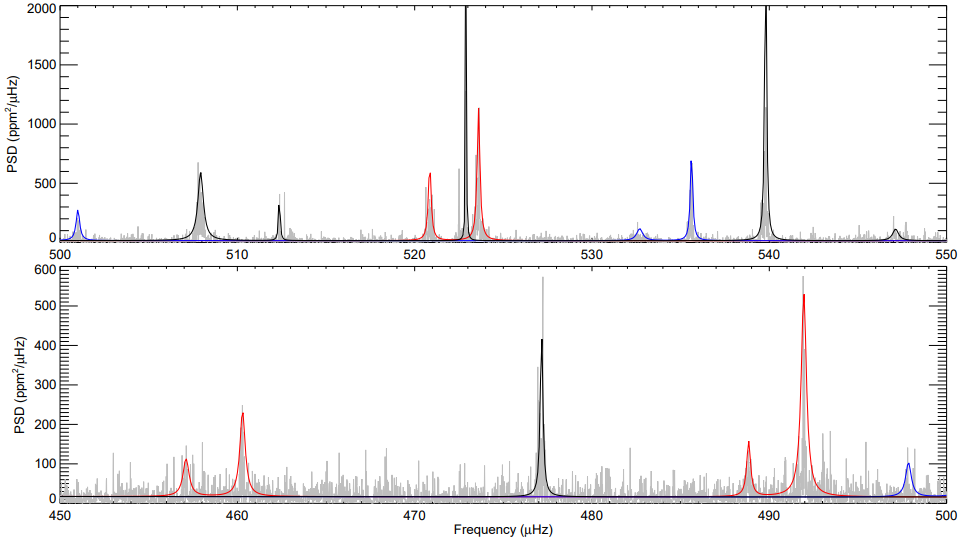
\includegraphics[width=\linewidth]{figs/power}
			Black lines are fit mixed modes ($l=1$). Red are star A $l=0,2$ modes. Blue are star B $l=0,2$ modes.
		\end{figure}
	}
	\frame {
		\frametitle{Modes}
		\begin{figure}
			\centering
			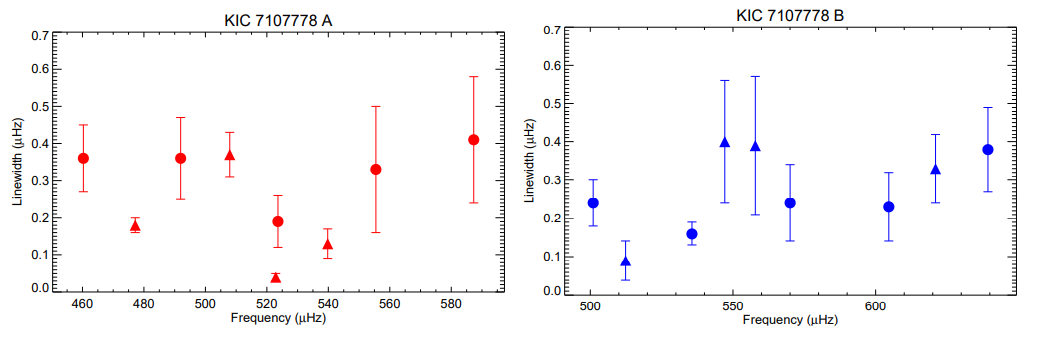
\includegraphics[width=\linewidth]{figs/modes}
			Circles represent $l=0$ and triangles represent $l=1$
		\end{figure}
	}
	\frame{
		\frametitle{Asteroseismic Analysis}
		Non-eclipsing; must estimate stellar parameters from power spectrum
		$$
		\frac{M}{M_\odot} \approx \left(\frac{\Delta \nu}{\Delta \nu_\odot}\right)^{-4} \left(\frac{\nu_{max}}{\nu_{max, \odot}}\right)^3 \left(\frac{T_{eff}}{T_{eff,\odot}} \right)^{3/2}
		$$
		This helps constrain \textit{MESA} modeling given the power spectra
	}
	\frame{
		\frametitle{\textit{MESA} Models, $l=0,2$}
		
		\begin{figure}
			\centering
			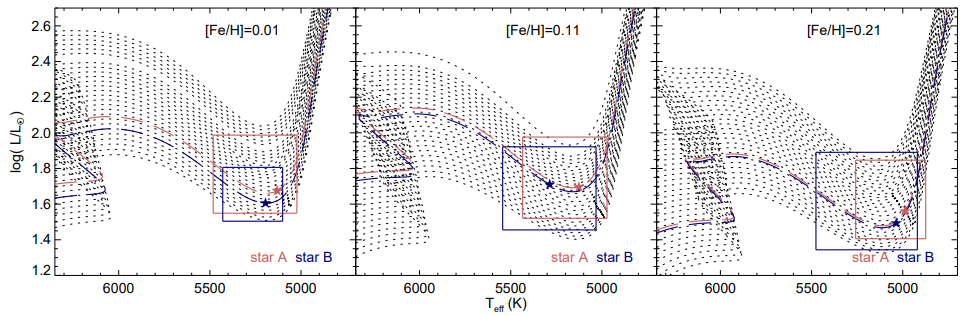
\includegraphics[width=\linewidth]{figs/HR}
		\end{figure}
		\begin{figure}
			\centering
			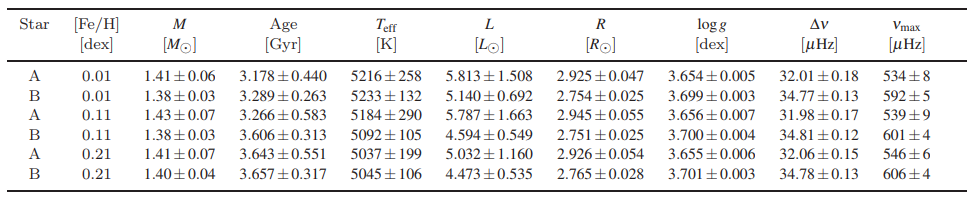
\includegraphics[width=\linewidth]{figs/HRresults}
		\end{figure}
	}
	\frame{
		\frametitle{\textit{MESA} Models, $l=1$}
		
		Mixed modes extremely sensitive to mass. Use bisection method to determine mass up to \SI{0.001}{M_\odot}
		\begin{figure}
			\centering
			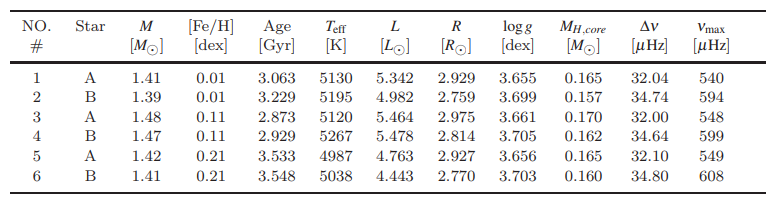
\includegraphics[width=.8\linewidth]{figs/HRresults2}
		\end{figure}
	}

	\frame {
		\frametitle{Conclusions}
		\begin{enumerate}
			\item KIC 7107778 is comprised of two subgiant stars with overlapping, solar-like power spectra
			\item The estimated stellar parameters of these stars show that they are nearly identical
			\begin{itemize}
				\item $M_A = \SI{1.42\pm0.06}{M_\odot}$, $M_B = \SI{1.39\pm0.03}{M_\odot}$
				\item $R_A = \SI{2.93\pm0.05}{R_\odot}$, $R_B = \SI{2.76\pm0.04}{R_\odot}$
				\item $t_A = \SI{3.32\pm0.54}{\giga yr}$, $t_B = \SI{3.51\pm 0.33}{\giga yr}$
			\end{itemize}
		\end{enumerate}
	}

\end{document}